\documentclass[xcolor=svgnames,aspectratio=169]{beamer}
\usepackage[utf8]{inputenc}
\usepackage{xcolor}
\usepackage{booktabs, comment} 
\usepackage{pgfpages}
\usepackage{csquotes}
\usepackage{amsmath}
\usepackage{tikz}
\usepackage{forest}
\usetikzlibrary{petri,positioning,fit,trees,arrows.meta}
\usetikzlibrary{decorations.pathmorphing,decorations.pathreplacing}
\usepackage{graphicx}
\usepackage{tcolorbox}
\usepackage{colortbl}
\usetheme{Madrid}
\usepackage{nicefrac}
\usepackage{bbm}
%\usepackage[backend=biber,style=apa]{biblatex}
%\addbibresource{references.bib}


% COLORS 
\definecolor{mqred}{RGB}{166, 25, 46}
\definecolor{mqdeepred}{RGB}{118, 35, 47}
\definecolor{mqgray}{RGB}{55, 58, 54}
\definecolor{mqlightgray}{RGB}{237, 235, 229}
\definecolor{mqmagenta}{RGB}{198, 0, 126}
\definecolor{darkgreen}{rgb}{0.0,0.5,0.0}
\definecolor{lightgreen}{rgb}{0.0,0.7,0.0}   % brighter green
\definecolor{mediumgreen}{rgb}{0.0,0.6,0.0}  % in between
% Muted colors
\definecolor{dark-blue}{RGB}{60, 85, 120}       % Slightly darker muted dark blue
\definecolor{darkred}{RGB}{120, 60, 60}        % Slightly darker muted dark red
\definecolor{light-gray}{RGB}{245,245,245}  % very light gray
\definecolor{mid-gray}{RGB}{230,230,230} % slightly darker gray
\definecolor{darkgreen}{rgb}{0.0,0.4,0.15} % dark green (used in TikZ labels)

% beamer theme
\usecolortheme[named=dark-blue]{structure}
\setbeamercolor{title in head/foot}{bg=mqlightgray, fg=mqgray}
\setbeamercolor{author in head/foot}{bg=dark-blue}
\setbeamercolor{page number in head/foot}{bg=dark-blue, fg=white}

% FOOTNOTE ARRANGEMENTS

\makeatletter
\setbeamertemplate{footline}{
  \leavevmode%
  \hbox{%
  \begin{beamercolorbox}[wd=.2\paperwidth,ht=2.25ex,dp=1ex,center]{author in head/foot}%
    \usebeamerfont{author in head/foot}\insertshortauthor\expandafter\ifblank\expandafter{\beamer@shortinstitute}{}{~~(\insertshortinstitute)}
  \end{beamercolorbox}%
  \begin{beamercolorbox}[wd=.6\paperwidth,ht=2.25ex,dp=1ex,center]{title in head/foot}%
    \usebeamerfont{title in head/foot}\insertshorttitle
  \end{beamercolorbox}%
  \begin{beamercolorbox}[wd=.2\paperwidth,ht=2.25ex,dp=1ex,center]{page number in head/foot}%
    \usebeamerfont{page number in head/foot}\insertframenumber{} / \inserttotalframenumber 
  \end{beamercolorbox}}%
  \vskip0pt%
}
\makeatother
\beamertemplatenavigationsymbolsempty


% TITLE, AUTHORS, INSTITUTE, DATE

\title[GNNExplainer : Generating Explanations for GNNs]{\large{GNNExplainer: Generating Explanations for Graph Neural Networks} \\
\small{\textit{Ying et al.}}}
\author[A. Scheid]{Arion Scheid}
\institute[TUWien]{TU Wien}
\date{May 2026}


\begin{document}

\begin{frame}
    \titlepage
\end{frame}

\begin{frame}{Motivation}
    \begin{itemize}
        \item GNNs:
        \begin{itemize}
            \item Powerful for learning graph structured data
            \item Incorporate graph structure \textbf{and} feature information $\Rightarrow$ Complex models
            \item Lack of interpretability
        \end{itemize}
        \item Goal: Generate explanations!
        \begin{itemize}
            \item Increases trust in model
            \item Improves transparency (for fairness, privacy, safety)
            \item Helps identify network characteristics, systematic patterns of mistakes
        \end{itemize}
        \item Problem: GNNs are complex, so explanations are hard!
    \end{itemize}
\end{frame}


\begin{frame}{Explanation Idea}
    \begin{figure}[H]
    \centering
    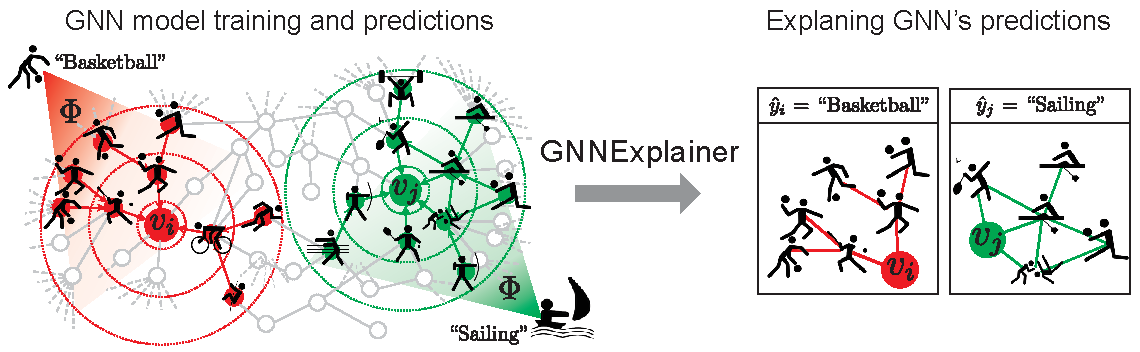
\includegraphics[width=0.8\textwidth]{figs/explainer-introduction_v2.pdf}
    \caption{Explaining hobby predictions with social network graph\footnote{Ying et al., GNNExplainer: Generating Explanations for Graph Neural Networks, 2019}}
    \end{figure}
\end{frame}

\begin{frame}{Computation graph}
    \begin{figure}[H]
    \centering
    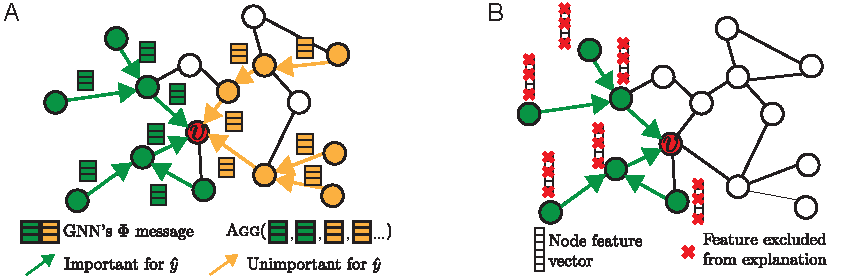
\includegraphics[width=0.8\textwidth]{figs/motivation-node-features.pdf}
    \caption{Explanations consist of identifying relevant nodes and features \footnote{Ying et al., GNNExplainer: Generating Explanations for Graph Neural Networks, 2019}}
    \end{figure}
\end{frame}


%%%%%%%%%%%%%%%%%%%%%%%%%%%%%%%%%%%%%%%%%%%%%%%%%%%%%%%%%%%%%%%%%%%%%
\section{Background: Information Theory}

\begin{frame}{Notation and setup}
    Throughout this presentation we use the following notation:
    \begin{itemize}
        \item $G = (V, E)$ --- a graph with node set $V$ and edge set $E$
        \item $X \in \mathbb{R}^{|V| \times d}$ --- node feature matrix ($d$ features per node)
        \item $\Phi$ --- a \textbf{trained, frozen} GNN (weights are fixed during explanation)
        \item $\hat{y} = \Phi(G, X)_v$ --- the GNN's predicted label for node $v$
        \item $G_c(v)$ --- the \textbf{computation graph} of node $v$: the $L$-hop neighbourhood that the $L$-layer GNN aggregates over to produce $\hat{y}$
        \item $A_c$ --- the adjacency matrix of $G_c(v)$
        \item $Y$ --- the predicted label viewed as a \textbf{random variable} (captures the GNN's softmax distribution over classes $1, \dots, C$)
    \end{itemize}
    \vspace{4pt}
    \textbf{Goal:} Find a small subgraph $G_S \subseteq G_c$ and a feature subset $X_S \subseteq X$ that are most important for the prediction $\hat{y}$.
\end{frame}

\begin{frame}{Entropy --- measuring uncertainty}
    \textbf{Shannon entropy} measures the uncertainty of a discrete random variable $Y$ with possible outcomes $\{1, \dots, C\}$:
    \begin{equation}
        H(Y) \;=\; -\sum_{c=1}^{C} P(Y=c)\,\log P(Y=c).
    \end{equation}
    \begin{columns}[T]
    \begin{column}{0.55\textwidth}
        \textbf{Properties:}
        \begin{itemize}
            \item $H(Y) \geq 0$; equals $0$ only when one outcome has probability $1$ (no uncertainty).
            \item Maximized when $Y$ is uniform, i.e.\ $P(Y=c)=\nicefrac{1}{C}$ for all $c$.
        \end{itemize}
        \textbf{Example ($C=3$ classes):}
        \begin{itemize}
            \item Confident: $P = (0.9, 0.05, 0.05)$ $\Rightarrow$ $H \approx 0.47$
            \item Uncertain: $P = (0.33, 0.33, 0.34)$ $\Rightarrow$ $H \approx 1.10$
        \end{itemize}
    \end{column}
    \begin{column}{0.42\textwidth}
        \centering
        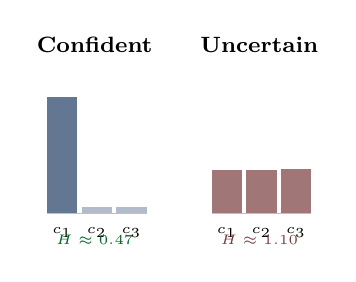
\begin{tikzpicture}[scale=0.55]
            % Confident prediction
            \node[anchor=south, font=\footnotesize\bfseries] at (1.1, 3.5) {Confident};
            \fill[dark-blue!80] (0,0) rectangle (0.7,2.7);     % 0.9
            \fill[dark-blue!40] (0.8,0) rectangle (1.5,0.15);  % 0.05
            \fill[dark-blue!40] (1.6,0) rectangle (2.3,0.15);  % 0.05
            \draw[gray!50] (0,0) -- (2.3,0);
            \node[font=\tiny, anchor=north] at (0.35,-0.1) {$c_1$};
            \node[font=\tiny, anchor=north] at (1.15,-0.1) {$c_2$};
            \node[font=\tiny, anchor=north] at (1.95,-0.1) {$c_3$};
            \node[font=\tiny, darkgreen] at (1.1, -0.6) {$H \approx 0.47$};
            % Uncertain prediction
            \begin{scope}[xshift=3.8cm]
                \node[anchor=south, font=\footnotesize\bfseries] at (1.1, 3.5) {Uncertain};
                \fill[darkred!70] (0,0) rectangle (0.7,1.0);    % 0.33
                \fill[darkred!70] (0.8,0) rectangle (1.5,1.0);  % 0.33
                \fill[darkred!70] (1.6,0) rectangle (2.3,1.02); % 0.34
                \draw[gray!50] (0,0) -- (2.3,0);
                \node[font=\tiny, anchor=north] at (0.35,-0.1) {$c_1$};
                \node[font=\tiny, anchor=north] at (1.15,-0.1) {$c_2$};
                \node[font=\tiny, anchor=north] at (1.95,-0.1) {$c_3$};
                \node[font=\tiny, darkred] at (1.1, -0.6) {$H \approx 1.10$};
            \end{scope}
        \end{tikzpicture}
    \end{column}
    \end{columns}
\end{frame}

\begin{frame}{Conditional entropy and mutual information}
    \textbf{Conditional entropy} --- residual uncertainty in $Y$ \emph{after} observing evidence $Z$:
    \begin{equation}
        H(Y \mid Z) \;=\; -\sum_{c=1}^{C} P(Y=c \mid Z)\,\log P(Y=c \mid Z).
    \end{equation}
    Conditioning on informative evidence reduces entropy: $H(Y \mid Z) \leq H(Y)$.\\[6pt]
    \textbf{Mutual information} --- how much observing $Z$ reduces our uncertainty about $Y$:
    \begin{equation}
        \operatorname{MI}(Y;\, Z) \;=\; H(Y) \;-\; H(Y \mid Z) \;\geq\; 0.
    \end{equation}
    \begin{center}
    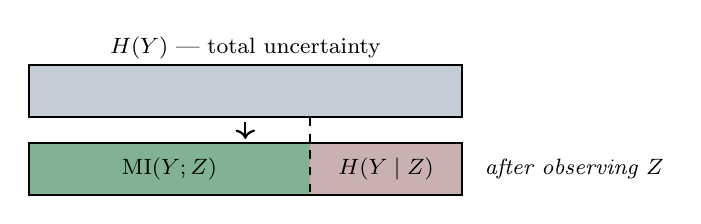
\begin{tikzpicture}[scale=0.55]
        % Full bar (H(Y))
        \fill[dark-blue!30] (0,0) rectangle (10, 1.2);
        \draw[thick] (0,0) rectangle (10,1.2);
        \node[font=\footnotesize] at (5, 1.6) {$H(Y)$ --- total uncertainty};
        % Split: MI and H(Y|Z)
        \fill[darkgreen!50] (0,-1.8) rectangle (6.5,-0.6);
        \fill[darkred!40] (6.5,-1.8) rectangle (10,-0.6);
        \draw[thick] (0,-1.8) rectangle (10,-0.6);
        \draw[thick, dashed] (6.5,0) -- (6.5,-1.8);
        \node[font=\footnotesize] at (3.25,-1.2) {$\operatorname{MI}(Y; Z)$};
        \node[font=\footnotesize] at (8.25,-1.2) {$H(Y \mid Z)$};
        \node[font=\footnotesize, anchor=west] at (10.3,-1.2) {\textit{after observing $Z$}};
        % Arrow
        \draw[->, thick] (5, -0.1) -- (5, -0.5);
    \end{tikzpicture}
    \end{center}
    \vspace{2pt}
    \textbf{Key insight:} A good explanation $Z = (G_S, X_S)$ should have \emph{high} MI --- observing it should make the prediction nearly certain (low $H(Y \mid Z)$).
\end{frame}

\begin{frame}{Intuition: how subgraph choice affects the prediction}
    \centering
    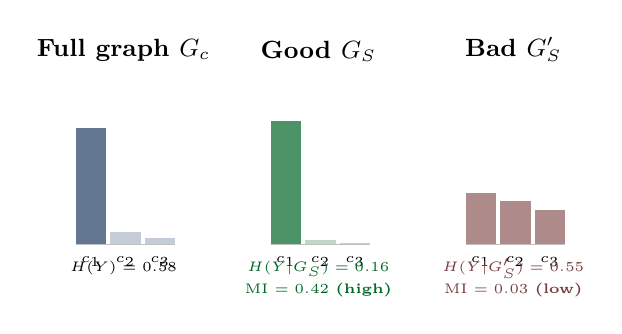
\begin{tikzpicture}[scale=0.55]
        % Full graph
        \node[font=\small\bfseries, anchor=south] at (1.1, 4.0) {Full graph $G_c$};
        \fill[dark-blue!80] (0,0) rectangle (0.7,2.7);
        \fill[dark-blue!30] (0.8,0) rectangle (1.5,0.3);
        \fill[dark-blue!30] (1.6,0) rectangle (2.3,0.15);
        \draw[gray!50] (0,0) -- (2.3,0);
        \node[font=\tiny, anchor=north] at (0.35,-0.05) {$c_1$};
        \node[font=\tiny, anchor=north] at (1.15,-0.05) {$c_2$};
        \node[font=\tiny, anchor=north] at (1.95,-0.05) {$c_3$};
        \node[font=\tiny] at (1.1, -0.55) {$H(Y) = 0.58$};
        % Good subgraph
        \begin{scope}[xshift=4.5cm]
            \node[font=\small\bfseries, anchor=south] at (1.1, 4.0) {Good $G_S$};
            \fill[darkgreen!70] (0,0) rectangle (0.7,2.85);
            \fill[darkgreen!25] (0.8,0) rectangle (1.5,0.1);
            \fill[darkgreen!25] (1.6,0) rectangle (2.3,0.05);
            \draw[gray!50] (0,0) -- (2.3,0);
            \node[font=\tiny, anchor=north] at (0.35,-0.05) {$c_1$};
            \node[font=\tiny, anchor=north] at (1.15,-0.05) {$c_2$};
            \node[font=\tiny, anchor=north] at (1.95,-0.05) {$c_3$};
            \node[font=\tiny, darkgreen] at (1.1, -0.55) {$H(Y|G_S) = 0.16$};
            \node[font=\tiny, darkgreen] at (1.1, -1.05) {MI $= 0.42$ \textbf{(high)}};
        \end{scope}
        % Bad subgraph
        \begin{scope}[xshift=9.0cm]
            \node[font=\small\bfseries, anchor=south] at (1.1, 4.0) {Bad $G_S'$};
            \fill[darkred!60] (0,0) rectangle (0.7,1.2);
            \fill[darkred!60] (0.8,0) rectangle (1.5,1.0);
            \fill[darkred!60] (1.6,0) rectangle (2.3,0.8);
            \draw[gray!50] (0,0) -- (2.3,0);
            \node[font=\tiny, anchor=north] at (0.35,-0.05) {$c_1$};
            \node[font=\tiny, anchor=north] at (1.15,-0.05) {$c_2$};
            \node[font=\tiny, anchor=north] at (1.95,-0.05) {$c_3$};
            \node[font=\tiny, darkred] at (1.1, -0.55) {$H(Y|G_S') = 0.55$};
            \node[font=\tiny, darkred] at (1.1, -1.05) {MI $= 0.03$ \textbf{(low)}};
        \end{scope}
    \end{tikzpicture}
    \vspace{6pt}

    \begin{itemize}
        \item \textbf{Good subgraph} $G_S$: contains the relevant structure $\Rightarrow$ GNN remains confident $\Rightarrow$ low $H(Y \mid G_S)$, high MI.
        \item \textbf{Bad subgraph} $G_S'$: misses key edges $\Rightarrow$ GNN becomes uncertain $\Rightarrow$ high $H(Y \mid G_S')$, low MI.
    \end{itemize}
\end{frame}

%%%%%%%%%%%%%%%%%%%%%%%%%%%%%%%%%%%%%%%%%%%%%%%%%%%%%%%%%%%%%%%%%%%%%
\section{Perturbation-based explanations}

\begin{frame}{Formal objective: maximize mutual information}
    For node $v$ with computation graph $G_c$, find the subgraph $G_S \subseteq G_c$ and features $X_S$ that maximize MI with the prediction:
    \begin{equation}
        \max_{G_S,\, X_S} \;\operatorname{MI}\!\left(Y,\; (G_S, X_S)\right) \;=\; \underbrace{H(Y)}_{\text{constant}} \;-\; H(Y \mid G\!=\!G_S,\, X\!=\!X_S).
    \end{equation}
    Since $\Phi$ is frozen, $H(Y)$ is fixed.  Maximizing MI $\equiv$ minimizing conditional entropy:
    \begin{equation}
        \label{eq:cond_entropy}
        \min_{G_S,\, X_S} \; H(Y \mid G\!=\!G_S,\, X\!=\!X_S) \;=\; -\sum_{c=1}^{C}\, P_\Phi(Y\!=\!c \mid G_S, X_S)\;\log P_\Phi(Y\!=\!c \mid G_S, X_S).
    \end{equation}
    This treats $Y$ as a full random variable: the loss uses the \textbf{entire softmax distribution} over all $C$ classes.  It penalizes any residual uncertainty --- the GNN should be \emph{confident}, regardless of which class it favours.
\end{frame}

\begin{frame}{Class-specific formulation}
    In practice, we know the GNN's predicted label $\hat{y} = c^*$.  We can replace the full entropy with a \textbf{cross-entropy targeted at $c^*$}:
    \begin{equation}
        \label{eq:class_specific}
        \min_{G_S,\, X_S} \; -\sum_{c=1}^{C} \mathbbm{1}[\hat{y} = c]\;\log P_\Phi(Y\!=\!c \mid G_S, X_S) \;=\; -\log P_\Phi(Y\!=\!c^* \mid G_S, X_S).
    \end{equation}

    \begin{columns}[T]
    \begin{column}{0.48\textwidth}
        \textbf{Conditional entropy} (Eq.~\ref{eq:cond_entropy}):
        \begin{itemize}
            \item Uses full distribution over all $C$ classes
            \item Asks: ``Is the GNN confident?''
            \item Penalizes \emph{any} uncertainty
        \end{itemize}
    \end{column}
    \begin{column}{0.48\textwidth}
        \textbf{Class-specific} (Eq.~\ref{eq:class_specific}):
        \begin{itemize}
            \item Only looks at $P(Y\!=\!c^*)$
            \item Asks: ``Does $G_S$ support predicting $c^*$?''
            \item Used in practice by Ying et al.
        \end{itemize}
    \end{column}
    \end{columns}
    \vspace{6pt}
    Both formulations agree when the GNN is highly confident.  The class-specific form is simpler and directly interpretable as the standard \textbf{cross-entropy loss} used in classification.
\end{frame}

\begin{frame}{Continuous relaxation with learnable masks}
    Searching over all subsets $G_S \subseteq G_c$ is combinatorial ($2^{|E|}$ options). Instead, learn continuous masks:
    \begin{itemize}
        \item \textbf{Edge mask} $M \in \mathbb{R}^{|E|}$: one scalar per edge, passed through sigmoid $\sigma(\cdot)$ to obtain weights in $[0,1]$.
        The masked adjacency is $A_c \odot \sigma(M)$, where $\odot$ is element-wise multiplication.
        \item \textbf{Feature mask} $F \in [0,1]^{d}$: one scalar per feature dimension.
        The masked features are $X_S = X_c \odot F$ (features not selected are zeroed out).
    \end{itemize}
    \vspace{4pt}
    Substituting into the class-specific objective:
    \begin{equation}
        \label{eq:opt_node_class}
        \min_{M,\, F}  \;-\log P_\Phi\!\left(Y = \hat{y} \;\middle|\; G = A_c \odot \sigma(M),\; X = X_c \odot F\right).
    \end{equation}
    Both $M$ and $F$ are optimized jointly via gradient descent through the frozen GNN $\Phi$.
\end{frame}

\begin{frame}{Regularization}
    The raw objective (Eq.~\ref{eq:opt_node_class}) can produce dense, uninterpretable masks. Regularization terms encourage \textbf{sparse} and \textbf{discrete} explanations:
    \begin{equation}
        \label{eq:full_loss}
        \mathcal{L} = \underbrace{-\log P_\Phi(Y\!=\!\hat{y} \mid A_c \odot \sigma(M),\, X_c \odot F)}_{\text{cross-entropy (fidelity)}}
        + \lambda_1 \underbrace{\|\sigma(M)\|_1}_{\text{size}}
        + \lambda_2 \underbrace{\sum_i H_{\mathrm{elt}}(\sigma(M_i))}_{\text{element-wise entropy}}
    \end{equation}
    where $H_{\mathrm{elt}}(p) = -p\log p - (1-p)\log(1-p)$ is the \textbf{binary entropy} of a single mask element.
    \vspace{4pt}
    \begin{itemize}
        \item \textbf{Size regularization} ($\|\sigma(M)\|_1$): penalizes the total ``mass'' of the mask, encouraging few edges to be selected $\Rightarrow$ compact explanation.
        \item \textbf{Element-wise entropy} ($H_{\mathrm{elt}}$): pushes each $\sigma(M_i)$ toward $0$ or $1$ (since $H_{\mathrm{elt}}$ is maximized at $0.5$ and zero at $0$ or $1$).  This discourages ambiguous, half-on mask values $\Rightarrow$ crisp, interpretable masks.
    \end{itemize}
\end{frame}

\begin{frame}{Perturbation-based explainers}
    \begin{figure}[H]
    \centering
    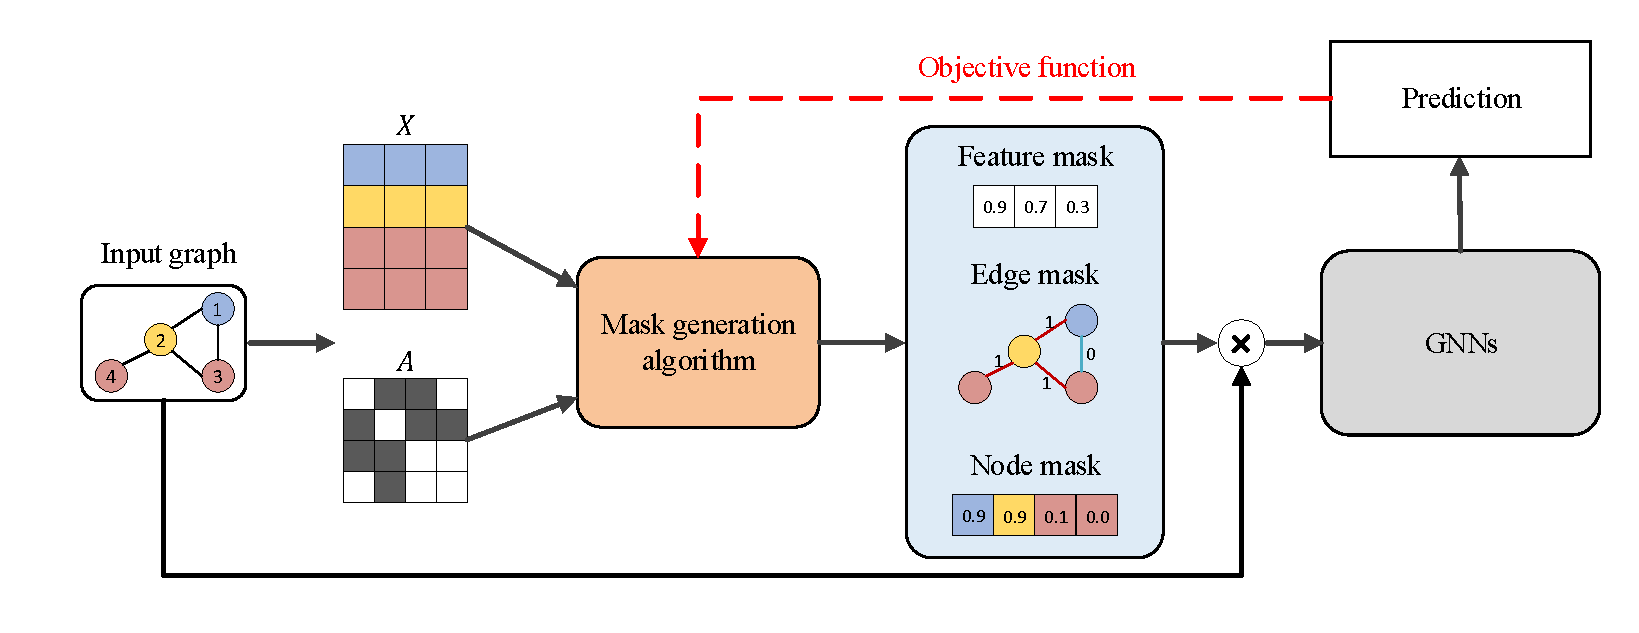
\includegraphics[width=0.8\textwidth]{figs/perturbation.pdf}
    \caption{General pipeline of perturbation-based explainers\footnote{Yuan et al., Explainability in Graph Neural Networks: A Taxonomic Survey, 2023}}
    \end{figure}
\end{frame}

\begin{comment}
%%%%%%%%%%%%%%%%%%%%%%%%%%%%%%%%%%%%%%%%%%%%%%%%%%%%%%%%%%%%%%%%%%%%%
\section{Other Methods}
\begin{frame}{Outline}
    \tableofcontents[currentsection]
\end{frame}

\begin{frame}{Taxonomy of explainers}
    \begin{figure}[H]
    \centering
    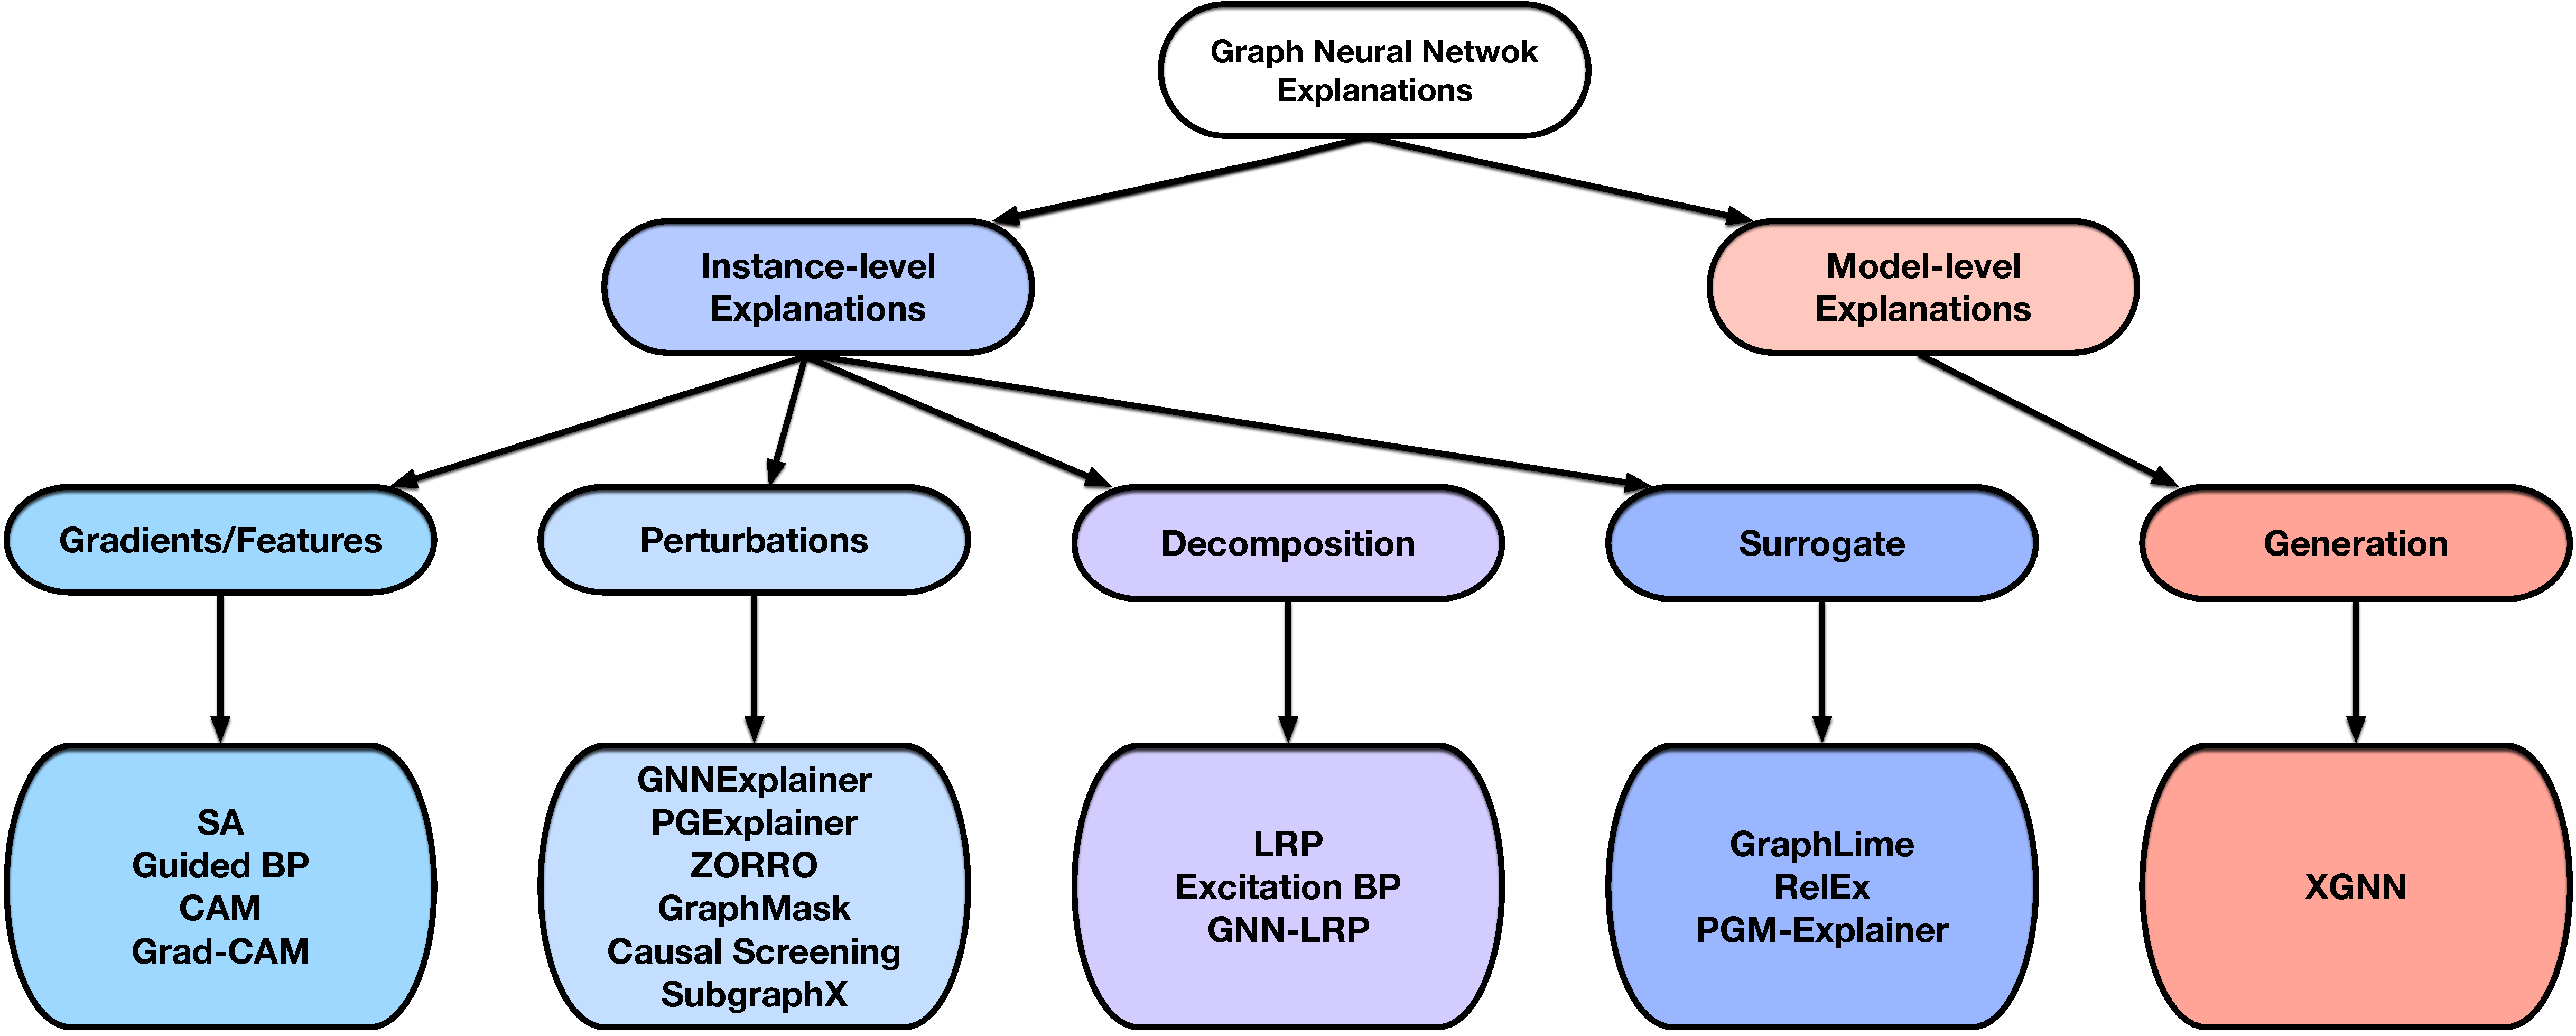
\includegraphics[width=0.8\textwidth]{figs/taxonomy.pdf}
    \caption{Taxonomy of GNN Explainers\footnote{Yuan et al., Explainability in Graph Neural Networks: A Taxonomic Survey, 2023}}
    \end{figure}
\end{frame}
\end{comment}



%%%%%%%%%%%%%%%%%%%%%%%%%%%%%%%%%%%%%%%%%%%%%%%%%%%%%%%%%%%%%%%%%%%%
\section{Evaluation}
\begin{frame}{Research Questions}
    \begin{itemize}
        \item Are the explanations sensible? 
        \begin{itemize}
            \item Can they identify ground truths?
            \item Can they make sense of real-world data?
        \end{itemize}
        \item How do other (newer) models compare?
        \item \textbf{Structural limitation:} Can gradient-based mask optimization get stuck?
    \end{itemize}
\end{frame}

\begin{frame}{Evaluation setup}
    For each target node, the explainer optimizes $\mathcal{L}$ (Eq.~\ref{eq:full_loss}), producing edge weights $\sigma(M_i) \in [0,1]$.
    We threshold at $0.5$: edges with $\sigma(M_i) > 0.5$ are \textbf{selected}; the rest are discarded.\\[4pt]

    \textbf{Accuracy} measures overall GNN classification quality (before explaining):
    \begin{equation}
        \mathrm{Acc} = \frac{\text{number of correctly classified nodes}}{\text{total nodes}}.
    \end{equation}

    To evaluate \emph{explanation} quality, we compare selected edges against ground-truth edges using \textbf{precision}, \textbf{recall}, and \textbf{F1 score}:
    \begin{equation}
        P = \frac{|\text{selected} \cap \text{ground truth}|}{|\text{selected}|}, \quad
        R = \frac{|\text{selected} \cap \text{ground truth}|}{|\text{ground truth}|}, \quad
        F_1 = \frac{2PR}{P+R}.
    \end{equation}
    \begin{itemize}
        \item $P$ --- of the edges the explainer highlights, how many are truly relevant?
        \item $R$ --- of the truly relevant edges, how many does the explainer find?
        \item $F_1$ --- harmonic mean; balances both (high only when both $P$ and $R$ are high).
    \end{itemize}
\end{frame}

\begin{frame}{F1 example: triangle in a small graph}
    \begin{columns}[T]
    \begin{column}{0.45\textwidth}
        \centering
        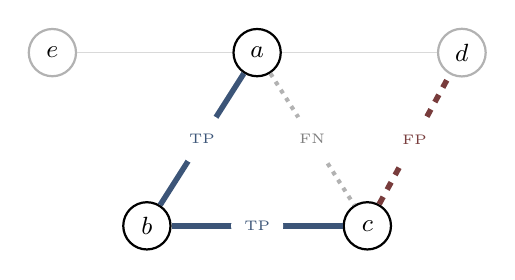
\begin{tikzpicture}[
            node distance=1.4cm,
            every node/.style={circle, draw, thick, minimum size=6mm, font=\small},
            gt/.style={line width=2pt, darkgreen},
            sel/.style={line width=2pt, dark-blue},
            fp/.style={line width=2pt, darkred, dashed},
            miss/.style={line width=1.5pt, gray!60, dotted},
        ]
            \node (A) at (0, 2.2) {$a$};
            \node (B) at (-1.4, 0) {$b$};
            \node (C) at (1.4, 0) {$c$};
            \node[draw=gray!60] (D) at (2.6, 2.2) {$d$};
            \node[draw=gray!60] (E) at (-2.6, 2.2) {$e$};

            % Ground truth triangle edges (selected correctly = TP)
            \draw[sel] (A) -- (B) node[midway, fill=white, draw=none, font=\tiny, text=dark-blue] {TP};
            \draw[sel] (B) -- (C) node[midway, fill=white, draw=none, font=\tiny, text=dark-blue] {TP};
            % Missed ground-truth edge (FN)
            \draw[miss] (A) -- (C) node[midway, fill=white, draw=none, font=\tiny, text=gray] {FN};
            % Spurious selected edge (FP)
            \draw[fp] (C) -- (D) node[midway, fill=white, draw=none, font=\tiny, text=darkred] {FP};
            % Non-selected, non-GT edges (background)
            \draw[gray!30, thin] (A) -- (E);
            \draw[gray!30, thin] (A) -- (D);
        \end{tikzpicture}

        \vspace{4pt}
        {\footnotesize Ground truth: triangle $\{a,b,c\}$ (3 edges).}
    \end{column}
    \begin{column}{0.52\textwidth}
        The explainer selects edges $\{a\text{-}b,\; b\text{-}c,\; c\text{-}d\}$.\\[6pt]
        \begin{tabular}{ll}
            \textcolor{dark-blue}{\textbf{TP}} (correct) & $a$-$b$, $b$-$c$ $\;\Rightarrow 2$ \\
            \textcolor{darkred}{\textbf{FP}} (spurious) & $c$-$d$ $\;\Rightarrow 1$ \\
            \textcolor{gray}{\textbf{FN}} (missed) & $a$-$c$ $\;\Rightarrow 1$ \\
        \end{tabular}
        \\[8pt]
        \begin{align*}
            P  &= \frac{2}{2+1} = 0.67 \\[2pt]
            R  &= \frac{2}{2+1} = 0.67 \\[2pt]
            F_1 &= \frac{2 \times 0.67 \times 0.67}{0.67 + 0.67} = 0.67
        \end{align*}

        \vspace{2pt}
        {\footnotesize A perfect explanation would recover all 3 triangle edges and nothing else $\Rightarrow$ $F_1 = 1.0$.}
    \end{column}
    \end{columns}
\end{frame}

\begin{frame}{Synthetic examples}
    \begin{figure}[H]
    \centering
    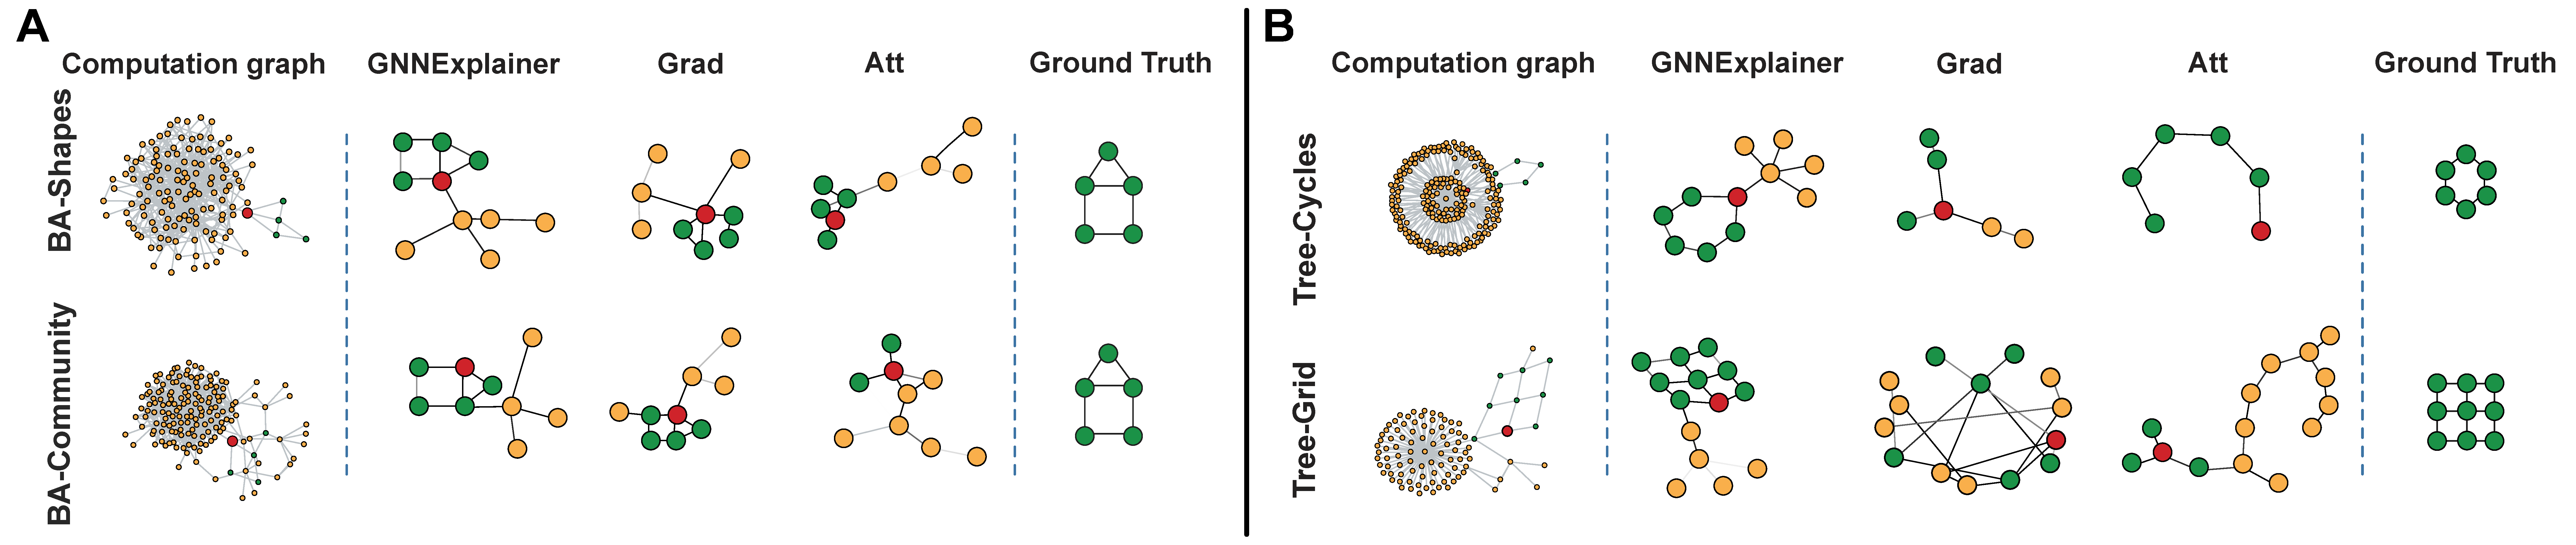
\includegraphics[width=0.8\textwidth]{figs/fig3-node-cls-v3.pdf}
    \caption{Examples with known ground truths for evaluation\footnote{Ying et al., GNNExplainer: Generating Explanations for Graph Neural Networks, 2019}}
    \end{figure}
\end{frame}

\begin{frame}{Real-world examples}
    \begin{figure}[H]
    \centering
    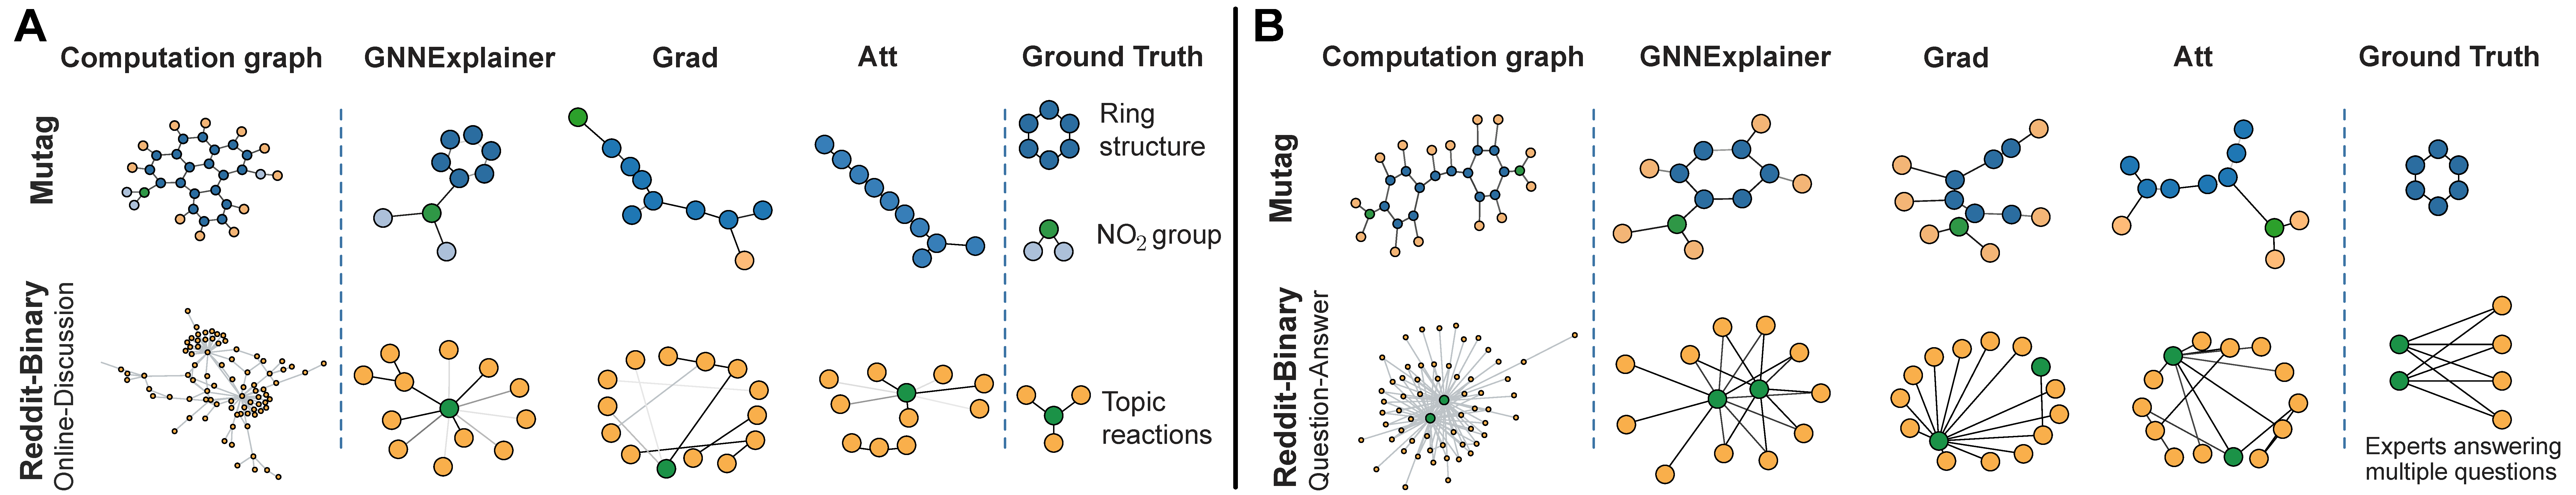
\includegraphics[width=0.8\textwidth]{figs/fig3-graph-cls-v2.pdf}
    \caption{Real-world examples for evaluation\footnote{Ying et al., GNNExplainer: Generating Explanations for Graph Neural Networks, 2019}}
    \end{figure}
\end{frame}

%%%%%%%%%%%%%%%%%%%%%%%%%%%%%%%%%%%%%%%%%%%%%%%%%%%%%%%%%%%%%%%%%%%%
\section{Limitation: Local Optima}

\begin{frame}{Local optima failure mode}
    \begin{itemize}
        \item Gradient descent finds the \emph{nearest} local minimum, not the global optimum
        \item Problem arises when sub-structures of the correct explanation are \emph{also} locally sufficient (i.e., already maintain high prediction confidence)
        \item Example: node in a $k$-clique embedded in sparse Erd\H{o}s-R\'enyi graph
        \begin{itemize}
            \item Erd\H{o}s-R\'enyi: random graph where each edge exists independently with probability $p$
            \item A triangle within the $k$-clique is already denser than the sparse background
            \item Optimizer stops at triangle --- a \emph{sub-clique local minimum}
        \end{itemize}
        \item Number of competing sub-optima grows \textbf{exponentially} with clique size $k$
    \end{itemize}
\end{frame}

\begin{frame}{Multi-size clique experiment}
    \begin{itemize}
        \item Novel benchmark: cliques of size 3, 4, 5 embedded in sparse Erd\H{o}s-R\'enyi graph ($n=200$, $p=0.02$)
        \item Binary labels (clique / non-clique); node features uniform $\Rightarrow$ GNN must rely on structure
        \item Results confirm local-optima failure:
    \end{itemize}
    \begin{center}
    \begin{tabular}{lccc}
        \toprule
        Clique size & F1 & Avg.\ expl.\ clique size \\
        \midrule
        $k=3$ (triangles) & 0.256 & 1.71 / 3 \\
        $k=4$             & 0.105 & 1.33 / 4 \\
        $k=5$             & 0.006 & 1.07 / 5 \\
        \bottomrule
    \end{tabular}
    \end{center}
    \vspace{4pt}
    \small F1 degrades sharply; optimizer almost always stops at a single edge (2-clique) for large cliques.
\end{frame}


%\section{References}
%\printbibliography

\end{document}
